\section{Optics}

\subsection{Target Variable Reconstruction Algorithm}
Reconstructing the target variables
$\delta_{tar}=\Delta p/p_0$, $x'_{tar}$, $y_{tar}$, and $y'_{tar}$
is an iterative process that makes use of optimized optics matrix elements
and polynomial combinations of $x_{tar}$ and focal plane variables
$x_{fp}$, $x'_{fp}$ $y_{fp}$, and $y'_{fp}$.

\begin{align} \label{eqn:optics_reconstruction}
    x'_{tar}     &= \sum_{ijklm} X'_{ijkml} x^i_{fp} x'^j_{fp} y^k_{fp} y'^l_{fp} x^m_{tar} \\
    y_{tar}      &= \sum_{ijklm} Y_{ijkml}  x^i_{fp} x'^j_{fp} y^k_{fp} y'^l_{fp} x^m_{tar} \\
    y'_{tar}     &= \sum_{ijklm} Y'_{ijkml} x^i_{fp} x'^j_{fp} y^k_{fp} y'^l_{fp} x^m_{tar} \\
    \delta_{tar} &= \sum_{ijklm} D_{ijkml}  x^i_{fp} x'^j_{fp} y^k_{fp} y'^l_{fp} x^m_{tar}
\end{align}

% TODO clean up wording here.
This iterative process entails the following steps:
\begin{enumerate}
    \item Estimate $x_{tar}$ from BPM and fast raster.
    \item Use optics matrices to estimate yptar, xptar, ytar.
    \item Correct these esimates for mispointing.
    \item Use the calculations outlined below to obtain a new estimate of $x_{tar}$.
    \item Return to Step 2 for some number of iterations, typically 6 or 7.
\end{enumerate}

% TODO: add a BCM/raster coordinate system to emphasize right-handed coordinates
\begin{figure}[!h]
    \centering
    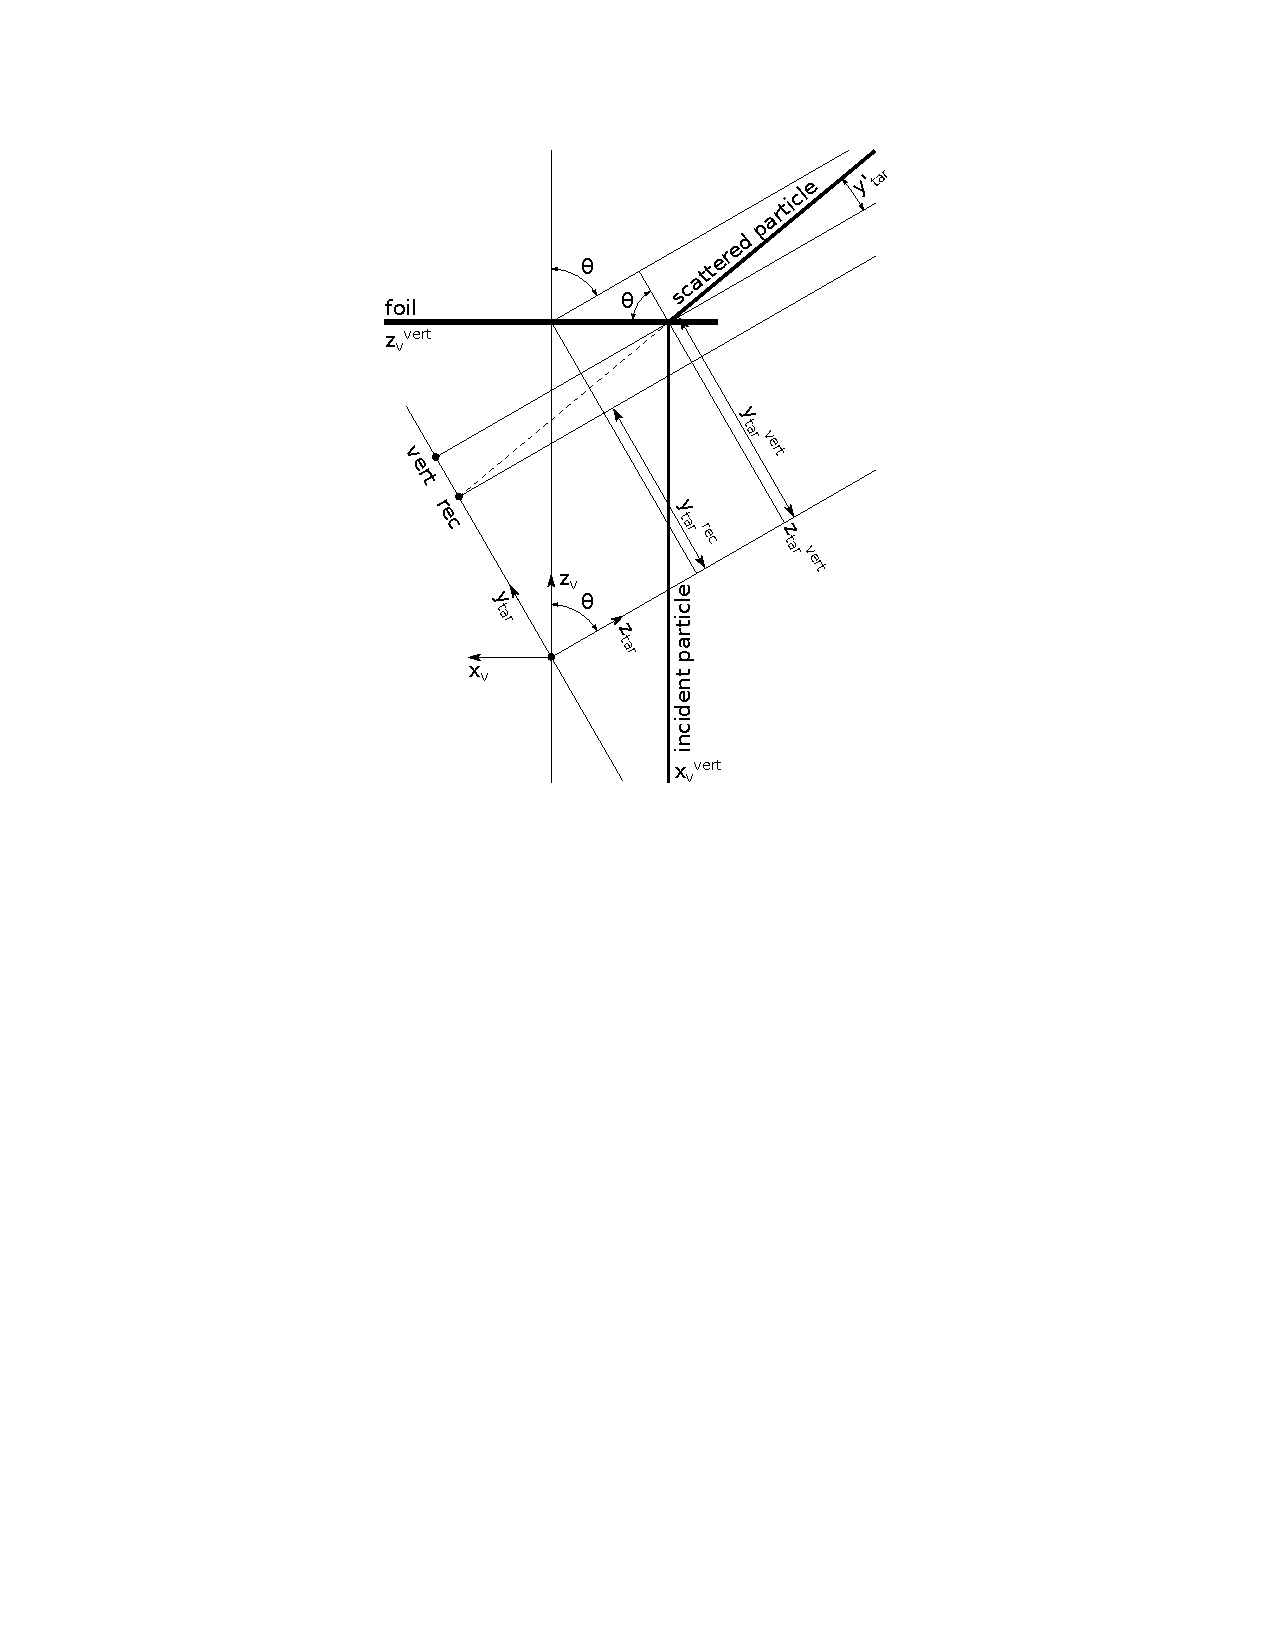
\includegraphics[width=0.6\textwidth]{chap4/optics_coordinates.pdf}
    \caption{
            Coordinate systems and distances relevant to reconstruction.
            The coordinates with subscript $v$ are in the target coordinate
            system,
            and the coordinates with subcript $tar$ are reconstructed
            coordinates in the spectrometer coordinate system.
            The label ``vert'' marks the projection of the interaction vertex
            onto the spectrometer coordinate system.
            The label ``rec'' marks the reconstructed point calculated by the
            optics matrices using equation~\ref{eqn:optics_reconstruction}.
            Figure reproduced from Ref~\cite{Bericic_2017}.
            }
    \label{fig:optics_coordinates}
\end{figure}

To derive these equations, consider Figure~\ref{fig:optics_coordinates} and
assume for now that the labeled distances are all known.
Assume, as a first estimate, that the $x^{vert}_{tar}$ coordinate in the
spectrometer coordinate system is given by the BPM and fast raster measurements
\begin{equation}
    x^{vert}_{tar} = -y^{beam} = -(y_0^{beam} - y_{fr})
\end{equation}

The reconstructed $y^{rec}_{tar}$ coordinate in the spectrometer coordinate
system is
\begin{equation} \label{eqn:yrectar}
    y^{rec}_{tar} = y^{vert}_{tar} - \frac{dy}{dz} z^{vert}_{tar}
                  = y^{vert}_{tar} - y'_{tar} z^{vert}_{tar}
\end{equation}

The vertex coordinates in the spectrometer coordinate system can be obtained
with a simple rotation from the target coordinate system
\begin{align} \label{eqn:yzverttar}
    y^{vert}_{tar} &= z^{vert}_v \sin\theta + x^{vert}_v \cos\theta \\
    z^{vert}_{tar} &= z^{vert}_v \cos\theta - x^{vert}_v \sin\theta
\end{align}

The $x^{vert}_{v}$ and $y^{vert}_{v}$ coordinates in the
target coordinate system are given by the BPM and fast raster
measurements\footnote{Recall that these use a right-handed coordinate system}
\begin{align}
    x^{vert}_v &= -x^{beam} = -(y_0^{beam} - x_{fr}) \\
    y^{vert}_v &= y^{beam} = y_0^{beam} - y_{fr}
\end{align}

Plugging equations~\ref{eqn:yzverttar} into equation~\ref{eqn:yrectar} and
solving for $z^{vert}_v$,
\begin{align}
    y^{rec}_{tar} &= (z^{vert}_v \sin\theta + x^{vert}_v \cos\theta) -
                     y'_{tar} (z^{vert}_v \cos\theta - y^{vert}_v \sin\theta) \\
                  &= (\sin\theta-y'_{tar}\cos\theta)z^{vert}_v +
                     (\cos\theta + y'_{tar} \sin\theta) x^{vert}_v \\
                  &= (\sin\theta-y'_{tar}\cos\theta)z^{vert}_v -
                     (\cos\theta + y'_{tar} \sin\theta) x^{beam}
\end{align}

\begin{equation}
    z^{vert}_v = \frac{y^{rec}_{tar} + x^{beam} (\cos\theta + y'_{tar} \sin\theta)}
                      {\sin\theta - y'_{tar}\cos\theta}.
\end{equation}

The above then provides a new estimate of $x^{rec}_{tar}$
\begin{equation}
    x^{rec}_{tar} = x^{vert}_{tar} - x'_{tar}z^{vert}_{tar} - x^{off}
\end{equation}

\subsection{Reconstruction Matrix Optimization}
The general process for optimizing optics matrix elements is outlined in
Ref~\cite{Bericic_2017}.
The optimization problem here is a on underdetermiend $\chi^2$ minimization
problem solved using Singular Value Decomposition (SVD).
The goal is to minimize the difference between ``true'' and reconstructed
values of $x'_{tar}$, $y_{tar}$, and $y'_{tar}$.
% TODO: clarify problem here is reconstructing 5 variables from 4;
% also xtar prop to xptar for given z
The collinearity of $x_{tar}$ and $\delta_{tar}$ makes optimization of matrix
elements with non-zero powers of $x_{tar}$ difficult.
As such, these elements are set to zero during the optimization steps and taken
from a COSY model during reconstruction.


Describe sieve/foil event selection here.


Consider a particular event $e$.
Let $o_e$ be one of the target variables $x'$, $y$, or $y'$ for this event,
$\hat{o}_e$ the ``true'' value of the variable,
and
$o^{rec}_e$ the estimate reconstructed
from the corresponding optics matrix $O_{ijkml}$.
For a set of matrices $O_{ijklm}$, $\chi^2$ is

\begin{align}
    \chi^2 &= \sum_e (\hat{o}_e - o^{rec}_e)^2 \\
           &= \sum_e \left( \hat{o}_e - \sum_{ijkml} O_{ijkml} x^i_{fp} x'^j_{fp} y^k_{fp} y'^l_{fp} x^m_{tar} \right)^2
\end{align}


Minimizing $\chi^2$, the derivative with respect to matrix elements
$O_{\bar{i}\bar{j}\bar{k}\bar{l}\bar{m}}$
for all combinations of particular indices
$\bar{i}$, $\bar{j}$, $\bar{k}$, $\bar{l}$, and $\bar{m}$
should be zero.
\begin{equation}
    \frac{d\chi^2}{dO_{ijklm}}
    = -2 \sum_e \left( \hat{o}_e - \sum_{ijkml} O_{ijkml} x^i_{fp} x'^j_{fp} y^k_{fp} y'^l_{fp} x^m_{tar} \right)
      x^{\bar{i}}_{fp} x'^{\bar{j}}_{fp} y^{\bar{k}}_{fp} y'^{\bar{l}}_{fp} x^{\bar{m}}_{tar}
    = 0
\end{equation}

For compactness of notation, let
\begin{equation} \label{eqn:index_abbreviation}
    n = (i,j,k,l,m)
\end{equation}
\begin{equation}
    \lambda_n = x^{i}_{fp} x'^{j}_{fp} y^{k}_{fp} y'^{l}_{fp} x^{m}_{tar}
\end{equation}
\begin{equation}
    \Lambda^e = \sum_n O_n \lambda^e_n
\end{equation}

Note that $\Lambda^e$ can be separated into parts that are dependent on and
independent of $x_{tar}$, $\Lambda^e = \Lambda^e_{ind} + \Lambda^e_{dep}$
by limiting the sums to include either
only indices $n'\in\text{ind}$ with zero powers of $x_{tar}$.
or
only indices $n''\in\text{dep}$ with nonzero powers of $x_{tar}$.
Rewriting the condition for minimizing $\chi^2$ with these definitions,
\begin{align}
    0 &= \sum_e (\hat{o}_e - \Lambda^e) \lambda_{\bar{n}} \\
      &= \sum_e (\hat{o}_e - \Lambda^e_{dep} - \Lambda^e_{ind}) \lambda_{\bar{n}}
\end{align}

\begin{align}
    \sum_e (\hat{o}_e - \Lambda^e_{dep}) \lambda_{\bar{n}} &= \sum_e \Lambda^e_{ind} \lambda_{\bar{n}} \\
            &= \sum_e \sum_{n\in\text{ind}} O_n \lambda_n \lambda_{\bar{n}} \\
            &= \sum_{n\in\text{ind}} O_n \sum_e \lambda_n \lambda_{\bar{n}} \\
\end{align}


There is one equation of this form for each $x_{tar}$-independent term indexed
by $\bar{n}$.
Together, they can be written in matrix notation
\begin{equation}
    \vec{b} = A \vec{x}
\end{equation}
where the matrix and vector elements are
\begin{equation}
    A_{ij} = \sum_e \lambda_i \lambda_j
\end{equation}
\begin{equation}
    x_i = O_i
\end{equation}
\begin{equation}
    b_i = \sum_e(\hat{o}_e - \Lambda^e_{dep}) \lambda_i
\end{equation}
and $i$ and $j$ are both abbreviations of the full set of indices as defined in
equation~\ref{eqn:index_abbreviation}.
This is now a well-posed problem that can be solved using SVD.
Recall that the terms included in this optimization step are only the
$x_{tar}$-independent terms.
After SVD, the $x_{tar}$-dependent terms from COSY are reintroduced to form the
full matrix elements used in reconstruction.
